% !TEX root = ./main.tex
\chapter{Analysis and Design}
\label{analysis}

\subsection{About Presage2}
PRESAGE2 is a simulation platform for multi-nodal or Agent simulation of societies. The platform was built and is currently maintained by PhD students within Imperial. This platform enables the project to investigate the impact of agent design (such as household behaviour), network properties (constraints on access) and the physical environment on individual agent behaviour and long-term global network performance \cite{Presage2-Desc:2015}. In the case of this project, each Node/Agent can represent individuals, households, businesses or generators. 

\subsection{Implementing the Micro Grid in Presage2}
Using Presage2, a network akin to the simplified model in Figure \ref{fig:SimpleModel} will be created and simulated. The Agents are reprsented by the Circles labeled A-H, and the various demand/generation equipment connected on the outside of the network represent the properties the Agents are expected to have.

\begin{figure}[h!]
\centering
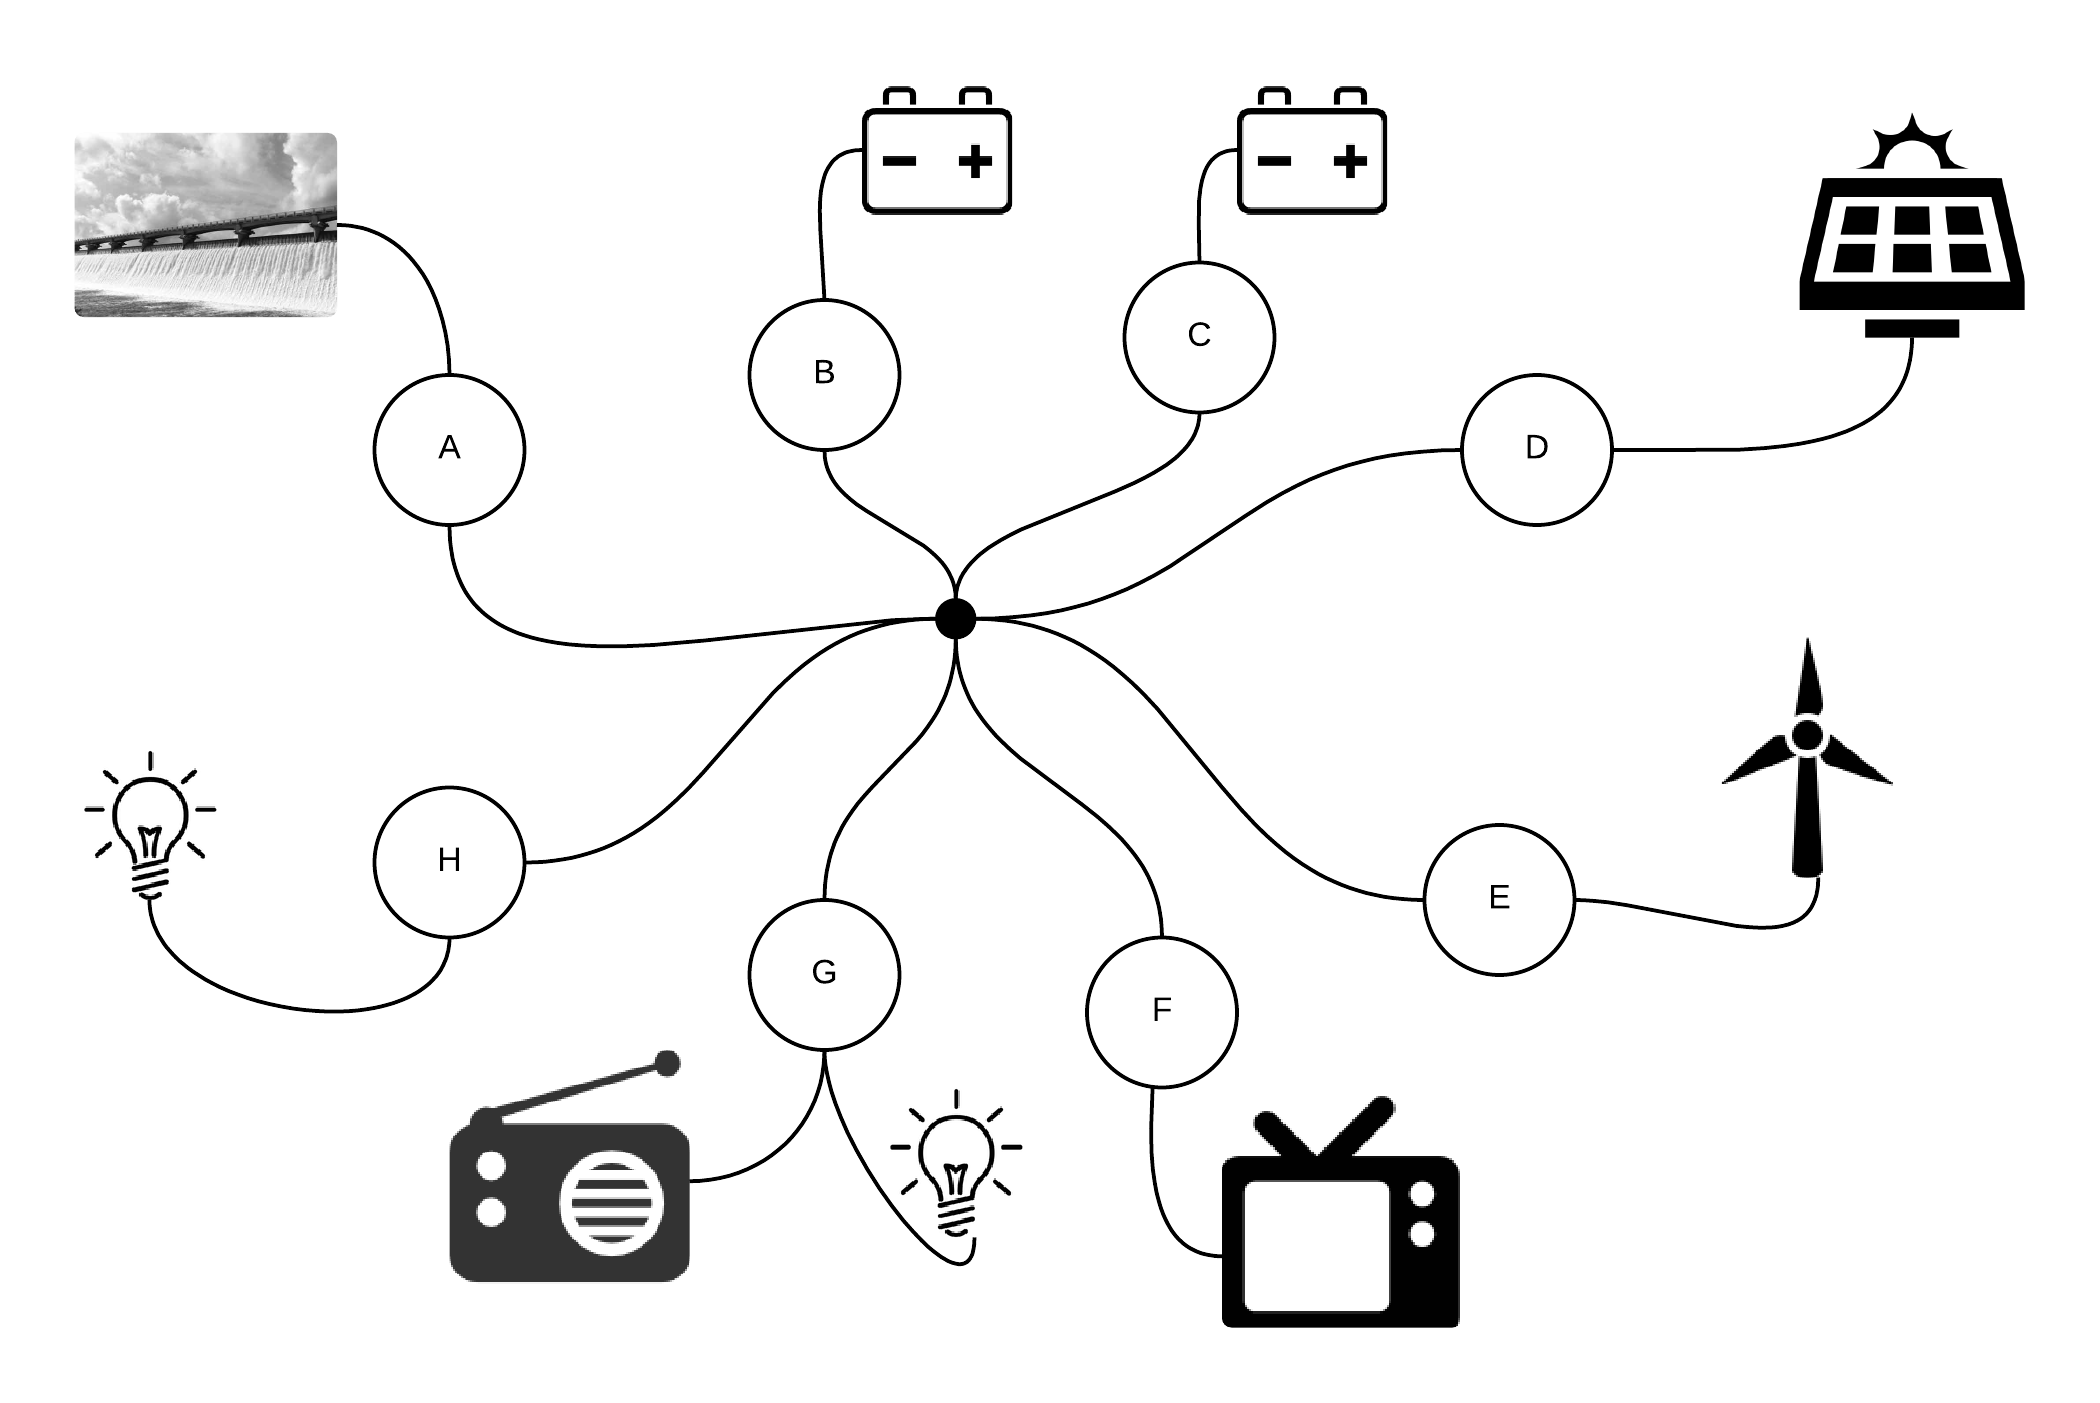
\includegraphics[scale=0.8]{Images/Model.png}
\caption{A simplified model diagram}
\label{fig:SimpleModel}
\end{figure}

In the immediate future, it is hoped that this tool could be used to aid the feasibility study of the Micro-Grid to be implemented in Rugaragara Falls. Should there be time, an energy trading platform will be designed and built based on the model created in this project to provide adequate electricity access to all members of the community. However, the energy trading platform would require a different design and implementation scheme which is not included in this report.

The sections below outlines the various properties each Agent must be able to take and how they could be implemented for the simulation scenario of rural communities in Rwanda. All of the properties must be allowed to exist on the same Agent during simulation.

\subsubsection{Agent Properties}

\paragraph{Generator}
Generators will be assumed to be generating power, and not draw any power from the Micro Grid. Four types of generator properties will be implemented in this simulation model: 

\begin{itemize}
  \item Hydro-electric - a constant source of energy based on a mixture of historical data and projections.
  \item Solar - a source of energy following the typical output profile of a solar panel connected to households.
  \item Wind - a source of energy which will be highly variable in output.
  \item Diesel - a constant source of energy.
\end{itemize}

With the power output of renewable sources of energy such as wind and solar being non-predictable in nature, one of two approach will need to be undertaken to model these sources:
\begin{itemize}
  \item A probabilistic generating factor is applied to the generators. This is a constant amount of power each solar panel or wind turbine is assumed to produce during some hours of the day that is to be determined. 
  
  \begin{itemize}
    \item * If this method is to be used, the model needs to be implemented in such a way to allow dynamic load-shedding and load-dumping.  
  \end{itemize}
  
  \item A probabilistic generation power output curve based on the least sunny / least windy days
  \begin{itemize}
    \item * If this method is to be used, sufficient weather and generation data will need to be obtained to implement this method
  \end{itemize}
\end{itemize}

More research will need to be conducted to look at which of the two methods will be more suitable in this application. Both methods are in use by distribution networks in the UK for assessing network congestion \cite{IPSA-web-constraint:2015}.

\paragraph{Demand}
The Demand property will only use electricity in the system. These represent households and businesses in the nearby village. Assumed demand curves will be produced from survey data of potential customers in the area for the initial testing. Should the survey data not be available for the area, a reasonable approximation will be made based a predicted usage habits of the wider local population.

It is anticipated that the final simulation will have a desired demand profile that each Demand-based agent will aim for by trading its allocated energy with other agents. However, the change in demand profile due to trading of energy must be able to satisfy the expected behavioral habits of the local inhabitants. These habits should include restrictions such as no trading during hours of sleep for households. What the habits will be, and how this will be implemented will be determined after some additional research into the area.

\paragraph{Storage}
The Storage property is a dynamic entity which can act as a generator or demand depending on the network utilisation and available power. These storage devices will be batteries of various types that will be connected to the network.

Storage properties will be attached to households which own battery boxes. The Storage property must have the capability to prioritise the allocation of its stored energy for certain Agents. For example, the energy output of Storage-only agents could be made to always prioritise the households they are attached to. If the battery box is communal or belongs to a centralised entity such as an e.quinox Energy Kiosk, then no priority will be attached.

\section{Simulation of the Micro Grid with Presage2}
With the village to be electrified implemented as a model with Presage2, studies will be conducted to determine the best allocation of resources to keep the customers in the village in a reasonably happy state. This would entail that every Agent will be able to consume all of its required energy consumption in the simulation period with a consumption/demand profile which follows all of the properties defined in the Demand property.

Further studies will also be conducted to determine the effects of varying the number of various properties in the network to create for example, a demand-heavy network or a generation-heavy network.  

\subsection{Model Assumptions}
With the Micro Grid model running under Normal Operation, a number of assumptions will be made to simplify the implementation of the model:
\begin{itemize}
\item No losses will be incurred by cables
\item All load on the network will be resistive
\item Only basic appliances such as phones, lights and fridges will be connected to the vast majority of households. A communal fridge-freezer and TV will be available at one of the households
\item Simulations will be run over a variable 1-7 day period
\end{itemize}

\section{Further work}
To facilitate the completion of this project, research will need to be carried out in the following areas:
\begin{itemize}
\item Continual updating of the Gantt Chart to track progress.
\item Research into additional sources of demand and load in rural developing countries and their typical usage to produce suitable realistic generation/demand curves for the simulation.
\item Consumer behaviour of the local population to determine a suitable demand curve, and the properties which are required to be part of the Demand property. e.quinox recently conducted a survey trip in January. The surveys will be used to produce potential demand profiles for the project.
\item Research into electricity generation and distribution infrastructure/equipment available in rural developing countries.
\item Number of households in the village will need to be determined to construct a realistic model.
\item The solar irradiation and photovoltaic cell generation profile for solar panels in developing countries will need to be reliably estimated. Preliminary research suggests an absence of data in this area. Data for Developed countries with similar climates could be used as an estimator.
\item Determine how to best estimate the output of a renewable source of energy dependent on the weather or time of day.
\item Typical storage sizes for battery storage units.
\item Design of Agents in Presage2 for the simulation.
\item Methods for implementing the simulation in Presage2.
\item A variety of rules and other management systems designed to efficiently allocate electricity access.
